% Chapter Template

\chapter{Introducción} % Main chapter title

\label{Chapter1} % Change X to a consecutive number; for referencing this chapter elsewhere, use \ref{ChapterX}

Las redes de telecomunicaciones crecen a medida que surgen nuevas tecnologías (redes inalámbricas \textit{4G} y \textit{5G}, \textit{WiMax}, \textit{LTE}, etc), seguido de la demanda en alza del ancho de banda por parte de los usuarios, requiriendo así cada vez mayor velocidad y mejor calidad de servicio. De esta forma, los operadores de red se ven obligados a aumentar la cantidad de dispositivos para satisfacer las necesidades de los usuarios, lo que constituye un desafío y un problema para los administradores de red, donde serán necesarios mecanismos de configuración que se adapten a las nuevas necesidades. 

Así, el paradigma actual de implementación de redes resulta difícil de adaptar a estos nuevos cambios en los requerimientos, por ejemplo:

\begin{itemize}     
    \item La complejidad y el tamaño de las redes ha crecido considerablemente, esto genera gran resistencia al cambio en los operadores ya que el riesgo de provocar una falla es mayor.

    \item Dependencia  de  un  fabricante,  la  falta  de  compatibilidad  entre  fabricantes fuerza a los operadores a quedar atados a los ciclos de diseño de un fabricante determinado y no les permite configurar la red de manera óptima dadas sus necesidades particulares. 
\end{itemize}

Desde el punto de vista de la infraestructura de comunicación, el mejor candidato para resolver este problema son las \textit{SDN} con la propuesta de separar el plano de control del plano de datos de los dispositivos, logrando una interfaz abierta entre ambos. De esta forma, se logra con \textit{SDN} que los equipos puedan ser vistos como una caja blanca, donde los mismos pueden relacionarse con independencia de fabricante. 

Por otra parte y desde el punto de vista de la gestión de la configuración, \textit{NETCONF} surge como una solución simple y estándar para la gestión de la configuración, donde el mismo proporciona a los operadores y administradores de red un \textit{framework} y un conjunto de métodos \textit{RPC} basados en codificación \textit{XML} para gestionar (instalar, modificar y borrar) la configuración de los elementos de red.

En el transcurso de este capítulo se introducen los aspectos más significativos del proyecto. Se comienza describiendo las motivaciones principales que han llevado al desarrollo de este trabajo. Luego, se expone el estado actual de las tecnologías directamente relacionadas, continuando con los objetivos planteados y finalizando con una descripción de la organización del texto.

\section{Motivación e importancia del proyecto}

Se exponen a continuación las razones principales que incentivaron la realización de este trabajo de fin de grado.

\begin{itemize}     
    \item Oportunidad de incursionar en el estudio de sistemas de administración de redes de vanguardia.
    \item La aplicación de los conocimientos adquiridos a lo largo de la carrera de Ingeniería en Computación.
    \item Posibilidad de desarrollar un sistema de administración de redes en su totalidad.
    \item Oportunidad de trabajar en un entorno con diversos dispositivos, presentes en las distintas capas de la red y destacando la presencia de un dispositivo óptico de transporte de red, el \textit{muxponder} de 40GB.
\end{itemize}
    
\section{Estado del arte} \label{Estado_Arte} %poner que es lo que hace y que es lo que nosotros agregamos o cambiamos

En la presente sección se hace un estudio del estado de las tecnologías directamente relacionadas al proyecto, con el objetivo de fijar un marco de comparación y diferenciar el trabajo realizado. Particularmente, se presenta una visión global de las implementaciones existentes más relevantes relacionadas a la administración de la configuración y al esquema de redes definidas por software.



% tesis granada% tesis granada% tesis granada% tesis granada% tesis granada
\subsubsection*{\textit{Protocol Efficiencies of NETCONF versus SNMP for Configuration Management Functions}}

En \parencite{netconfvssnmp} se presenta una comparación entre el protocolo \textit{NETCONF} y el protocolo \textit{SNMP}. Para ello, se conforma la topología que puede verse en la figura \ref{fig:netconfvssnmp1}, utilizando como agente \textit{NETCONF} y agente \textit{SNMP} la implementación 'ConfD' de Cisco.

\begin{figure}[H]
	\centering 
	\resizebox{0.60\textwidth}{!}{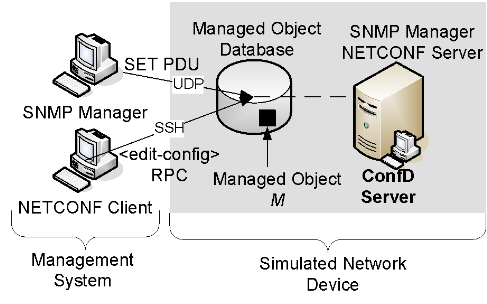
\includegraphics{Figures/netconfvssnmp1.png}}%
	\caption[Topología utilizada en las pruebas de.]{Topología utilizada en las pruebas de \parencite{netconfvssnmp}.}
	\label{fig:netconfvssnmp1}
\end{figure}

Las pruebas realizadas por los autores arrojan los resultados observados en la figura \ref{fig:netconfvssnmp2}, donde M representa la cantidad de operaciones a realizar por parte del servidor. Los autores mencionan que en los resultados obtenidos no se tiene en cuenta la carga que tienen los paquetes debido a la seguridad que ofrece el transporte \textit{SSH} por parte de \textit{NETCONF}, tampoco la carga que presenta \textit{TCP} (\textit{NETCONF}) frente a \textit{UDP} (\textit{SNMP}), entre otros.

\begin{figure}[th]
	\centering 
	\resizebox{1\textwidth}{!}{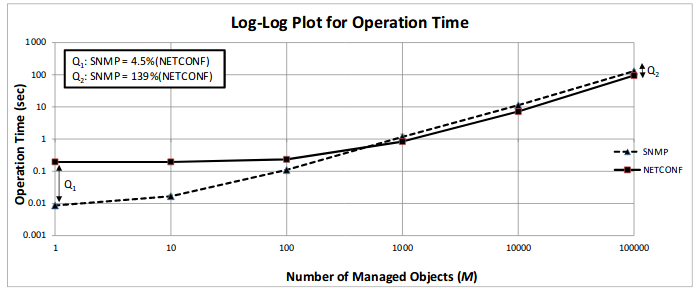
\includegraphics{Figures/netconfvssnmp2.png}}%
	\caption[Resultados obtenidos en.]{Resultados obtenidos en \parencite{netconfvssnmp}.}
	\label{fig:netconfvssnmp2}
\end{figure}

En las conclusiones de este artículo mencionan que \textit{NETCONF} es una clara alternativa a \textit{SNMP} en ámbitos de gestión de la configuración de la red. Además, destacan las bondades que presenta el protocolo \textit{NETCONF} frente a \textit{SNMP} para los proveedores de servicio como ser la seguridad de los mensajes mediante \textit{SSH}, la capacidad de revertir una configuración, el transporte de los mensajes mediante un protocolo orientado a la conexión, etc.



% tesis granada
\subsubsection*{\textit{Evaluating the Network Management Capabilities of YANG and NETCONF}}

En el artículo \parencite{netconfvstodos} se realiza un estudio de las diferentes alternativas existentes en el ámbito de la configuración y gestión de la red. A su vez, el autor desarrolla un prototipo de servidor \textit{NETCONF}. Los experimentos realizados por el autor tienen como objetivo determinar la capacidad que tienen los diferentes protocolos de gestión de configuración y monitoreo para adaptarse a entornos de \textit{SDN} y \textit{NFV}. 

Así, separa las pruebas realizadas en dos partes. En primer lugar, evalúa alternativas que permiten la configuración de un dispositivo de red. Luego, realiza un análisis de las alternativas relacionadas al monitoreo de un equipo de red.

La figura \ref{fig:netconfvstodos1} muestra una gráfica de los resultados obtenidos para el primer caso, donde concluye que \textit{NETCONF} se adapta bien a los entornos \textit{NFV} ya que se encuentra específicamente diseñado para la configuración de los equipos. Sin embargo, menciona que puede presentar dificultades adaptar el protocolo \textit{NETCONF} a entornos \textit{SDN} ya que no cumple estrictamente con el paradigma de las \textit{SDN}, donde el plano de control y el plano de datos se encuentran desacoplados íntegramente.

Por otra parte, la figura \ref{fig:netconfvstodos2} muestra el análisis para el segundo caso, en donde se evalúan protocolos y alternativas para el monitoreo de la red. En este caso, el autor menciona que si bien \textit{NETCONF} permite monitoreo en entornos \textit{NFV} y \textit{SDN}, el uso enfocado explícitamente a esta tarea no presenta mejores resultados que, por ejemplo, \textit{SNMP}.


\begin{figure}[H]
	\centering 
	\resizebox{0.8\textwidth}{!}{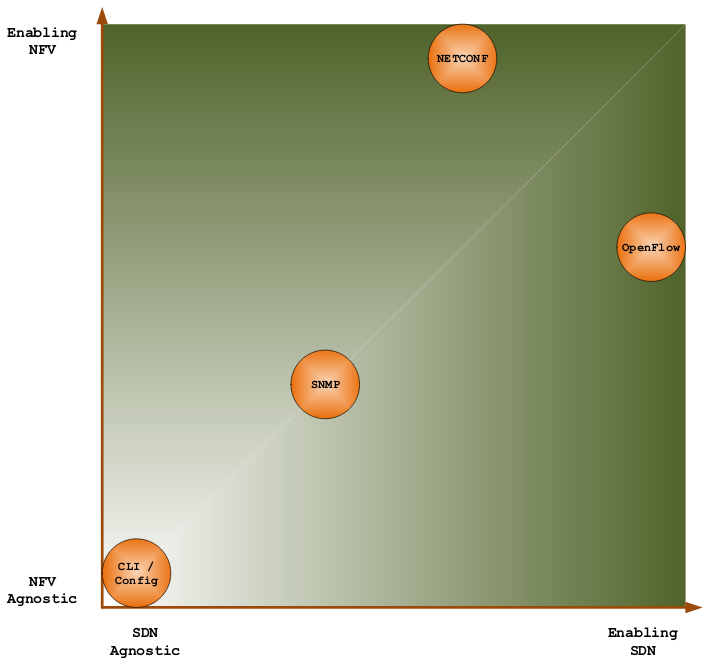
\includegraphics{Figures/netconfvstodos1.png}}%
	\caption[\textit{NETCONF} como protocolo para la administración.]{\textit{NETCONF} como protocolo para la administración \parencite{netconfvstodos}.}
	\label{fig:netconfvstodos1}
\end{figure}

\begin{figure}[H]
	\centering 
	\resizebox{0.8\textwidth}{!}{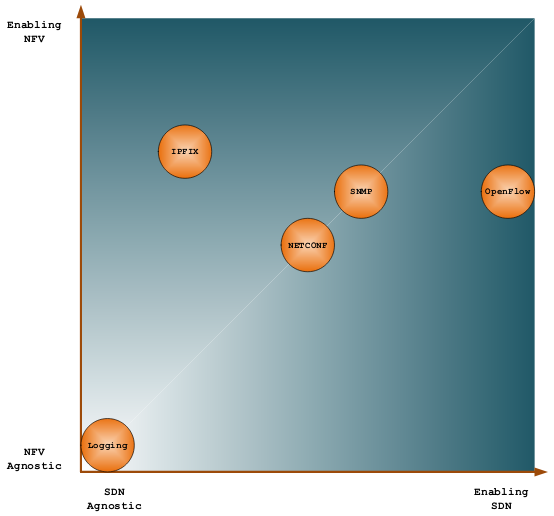
\includegraphics{Figures/netconfvstodos2.png}}%
	\caption[\textit{NETCONF} como protocolo para el monitoreo.]{\textit{NETCONF} como protocolo para el monitoreo \parencite{netconfvstodos}.}
	\label{fig:netconfvstodos2}
\end{figure}



% tesis granada% tesis granada% tesis granada% tesis granada% tesis granada
\subsubsection*{\textit{Control and Management of Transponders With NETCONF and YANG}}

El documento \parencite{netconfsddn} propone la utilización del protocolo de administración \textit{NETCONF} en un ambiente \textit{SDN} para administrar la configuración de un \textit{transponder}, sugiriendo un entorno como el que se puede ver en la figura \ref{fig:netconfsddn1}.


\begin{figure}[H]
	\centering 
	\resizebox{1\textwidth}{!}{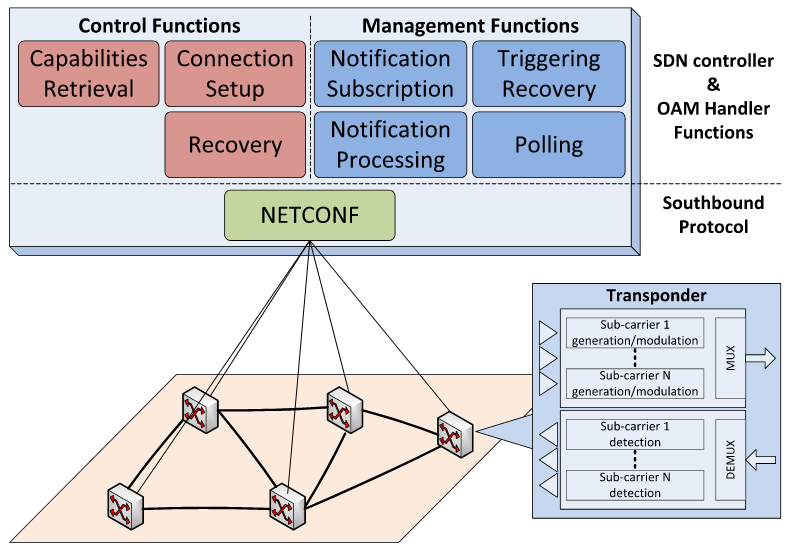
\includegraphics{Figures/netconfsddn1.png}}%
	\caption[Topología propuesta en.]{Topología propuesta en \parencite{netconfsddn}.}
	\label{fig:netconfsddn1}
\end{figure}

Sin embargo, finalmente realizan una demostración compuesta por dos \textit{transponders} y un \textit{switch}, los tres virtuales y sin utilización de algún controlador \textit{SDN}. Esta última topología se muestra en la figura \ref{fig:netconfsddn2}.


\begin{figure}[H]
	\centering 
	\resizebox{0.55\textwidth}{!}{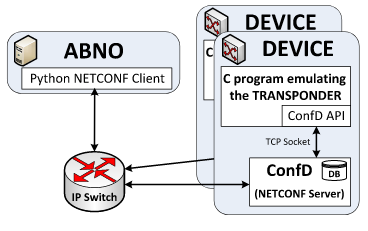
\includegraphics{Figures/netconfsddn2.png}}%
	\caption[Escenario propuesto para las pruebas en.]{Escenario propuesto para las pruebas en \parencite{netconfsddn}.}
	\label{fig:netconfsddn2}
\end{figure}

Los autores concluyen que \textit{NETCONF} como protocolo de gestión y \textit{YANG} como modelado de datos, son estándares viables para la configuración, gestión y monitoreo de los datos en dispositivos de red como los \textit{transponders}. 
Además, resaltan el alto rendimiento obtenido en sus pruebas para la configuración y monitoreo de los \textit{transponders} haciendo uso de estos protocolos. 


\section{Objetivos propuestos}

El objetivo general de este proyecto integrador es adquirir los conocimientos relacionados con administración de redes, particularmente con el esquema conocido como Redes Definidas por Software y el protocolo de administración de la configuración \textit{NETCONF}. Para esto, se propone usar como vehículo de prueba un entorno constituido por ambas tecnologías para lograr la administración y monitoreo del estado de un \textit{muxponder}. Se prestará particular atención al estudio y comparación de las diferentes opciones abiertas disponibles para la implementación del protocolo \textit{NETCONF}.

\subsection{Objetivos particulares}

Las tareas a realizar en este trabajo de fin de grado llevarán a:


\begin{itemize}
    \item Adquirir un amplio conocimiento de las tecnologías existentes en \textit{SDN}.   
    \item Tener un conocimiento acabado en el protocolo de administración de red \textit{NETCONF}.   
    \item Desarrollar una librería en el controlador \textit{SDN} que permita la comunicación, a través de \textit{NETCONF}, con un dispositivo óptico.   
    \item Compilar e instalar en un dispositivo óptico un agente del protocolo \textit{NETCONF} y una librería que relacione las variables de configuración y estado del dispositivo con dicho agente.   
    \item Desarrollar una aplicación de interfaz de usuario para administrar de manera simple los dispositivos de red.
\end{itemize}  
    
\section{Estructura del texto}

Aquí se listan los distintos capítulos que conforman el proyecto, presentando una breve descripción de su contenido. El escrito está compuesto por 6 capítulos, los apéndices y la bibliografía.


\begin{itemize}   
    \item \textbf{Capítulo 1 - Introducción:} Se exponen en este capítulo los aspectos más significativos del proyecto, donde se incluye las motivaciones que llevaron a realizar el mismo junto con una revisión del estado del arte relacionado y los objetivos propuestos para el trabajo de fin de grado.

    \item \textbf{Capítulo 2 - Marco teórico:} Aquí se abordan los conceptos necesarios para comprender las tecnologías utilizadas por el proyecto, además los mismos presentan una fundamentación para las posteriores implementaciones prácticas.

    \item \textbf{Capítulo 3 - Análisis de las tecnologías:} Se estudia y analiza en este capítulo todas las herramientas que permiten la implementación de las aplicaciones desarrolladas en este proyecto, abarcando tanto herramientas de software como de hardware.

    \item \textbf{Capítulo 4 - Diseño e implementación:} En este capítulo se abordan los procesos de diseño e implementación de todas las aplicaciones realizadas. Se presentan los requerimientos de las mismas y los diferentes diagramas realizados que explican el funcionamiento de cada pieza de software. 

    \item \textbf{Capítulo 5 - Validación y verificación:} Aquí, se exponen los diferentes casos de prueba desarrollados con el objetivo de validar y verificar que se cumplan los requerimientos de las diferentes aplicaciones.

    \item \textbf{Capítulo 6 - Conclusión:} Se presenta en este capítulo las conclusiones obtenidas tras la realización del trabajo, posibles vías de trabajos futuros y una apreciación personal del proceso abordado.
	
	\item \textbf{Apéndices:} En los apéndices se proporciona al lector un tutorial de como desplegar el entorno de trabajo y las aplicaciones desarrolladas en este proyecto.
    
    \item \textbf{Bibliografía:} En esta parte final del documento, se muestran todas las referencias que se han consultado para el desarrollo del proyecto.   
\end{itemize}

